\documentclass{beamer}
\mode<presentation> {
	
	% The Beamer class comes with a number of default slide themes
	% which change the colors and layouts of slides. Below this is a list
	% of all the themes, uncomment each in turn to see what they look like.
	
	%\usetheme{default}
	%\usetheme{AnnArbor}
	%\usetheme{Antibes}
	%\usetheme{Bergen}
	%\usetheme{Berkeley}
	%\usetheme{Berlin}
	%\usetheme{Boadilla}
	%\usetheme{CambridgeUS}
	%\usetheme{Copenhagen}
	%\usetheme{Darmstadt}
	%\usetheme{Dresden}
	%\usetheme{Frankfurt}
	%\usetheme{Goettingen}
	%\usetheme{Hannover}
	%\usetheme{Ilmenau}
	%\usetheme{JuanLesPins}
	%\usetheme{Luebeck}
	\usetheme{Madrid}
	%\usetheme{Malmoe}
	%\usetheme{Marburg}
	%\usetheme{Montpellier}
	%\usetheme{PaloAlto}
	%\usetheme{Pittsburgh}
	%\usetheme{Rochester}
	%\usetheme{Singapore}
	%\usetheme{Szeged}
	%\usetheme{Warsaw}
	
	% As well as themes, the Beamer class has a number of color themes
	% for any slide theme. Uncomment each of these in turn to see how it
	% changes the colors of your current slide theme.
	
	%\usecolortheme{albatross}
	%\usecolortheme{beaver}
	%\usecolortheme{beetle}
	%\usecolortheme{crane}
	%\usecolortheme{dolphin}
	%\usecolortheme{dove}
	%\usecolortheme{fly}
	%\usecolortheme{lily}
	%\usecolortheme{orchid}
	%\usecolortheme{rose}
	%\usecolortheme{seagull}
	%\usecolortheme{seahorse}
	%\usecolortheme{whale}
	%\usecolortheme{wolverine}
	
	%\setbeamertemplate{footline} % To remove the footer line in all slides uncomment this line
	%\setbeamertemplate{footline}[page number] % To replace the footer line in all slides with a simple slide count uncomment this line
	
	%\setbeamertemplate{navigation symbols}{} % To remove the navigation symbols from the bottom of all slides uncomment this line
}

\usepackage{graphicx} % Allows including images
\usepackage{booktabs} % Allows the use of \toprule, \midrule and \bottomrule in tables
\usepackage[utf8]{inputenc}
\usepackage[english,frenchb]{babel}
\usepackage[Algorithme]{algorithm}
\usepackage{algorithmic}
\usepackage{ulem}
\newcommand\redout{\bgroup\markoverwith
	{\textcolor{red}{\rule[0.5ex]{2pt}{0.8pt}}}\ULon}
\usepackage{tikz}
\usetikzlibrary{arrows}
\usetikzlibrary{calc,shapes}
\newcommand{\tikzmark}[1]{\tikz[overlay,remember picture] \node (#1) {};}
\def\checkmarkg{\tikz\fill[scale=0.4,black!30!green](0,.35) -- (.25,0) -- (1,.7) -- (.25,.15) -- cycle;}
\def\checkmarky{\tikz\fill[scale=0.4,black!30!yellow](0,.35) -- (.25,0) -- (1,.7) -- (.25,.15) -- cycle;}
\usepackage{amssymb}% http://ctan.org/pkg/amssymb
\usepackage{pifont}% http://ctan.org/pkg/pifont
\usepackage{color}
\usepackage{filecontents}
\usepackage{soul}
\usepackage{bibentry}
\usepackage{booktabs} % Allows the use of \toprule, 

\newcommand{\xmark}{\ding{55}}%
\newcommand\tab[1][1cm]{\hspace*{#1}}
\setbeamertemplate{items}[circle]

\newcommand\mynum[1]{%
	\usebeamercolor{enumerate item}%
	\tikzset{beameritem/.style={circle,inner sep=0,minimum size=2ex,text=enumerate item.bg,fill=enumerate item.fg,font=\footnotesize}}%
	\tikz[baseline=(n.base)]\node(n)[beameritem]{#1};%
}

\usepackage{caption}
\captionsetup{font=scriptsize,labelfont=scriptsize}

\makeatletter
\setbeamertemplate{headline}{%
	\begin{beamercolorbox}[ht=2.25ex,dp=3.75ex]{section in head/foot}
		\insertnavigation{\paperwidth}
	\end{beamercolorbox}%
}%
\makeatother
\newcommand{\CS}{\textsf{CS}}
\newcommand{\GPS}{\textsf{GPS}}
\newcommand{\GSS}{\textsf{GSS}}
\newcommand{\MADS}{\textsf{MADS}}
\newcommand{\IMFIL}{\textsf{IMFIL}}
\newcommand{\norm}[1]{\left\lVert#1\right\rVert}
\newcommand{\R}{\mathbb{R}}
%----------------------------------------------------------------------------------------
%	TITLE PAGE
%----------------------------------------------------------------------------------------

\title[Opportunisme et ordonnancement]{Opportunisme et ordonnancement en optimisation sans dérivées} % The short title appears at the bottom of every slide, the full title is only on the title page

\author{Loïc Anthony Sarrazin-Mc Cann} % Your name
\institute[GERAD] % Your institution as it will appear on the bottom of every slide, may be shorthand to save space
{
	École Polytechnique de Montréal \\ % Your institution for the title page
	\medskip
}
\date{\today} % Date, can be changed to a custom date

\begin{document}
	
\begin{frame}
	\titlepage % Print the title page as the first slide
\end{frame}

\begin{frame}
\frametitle{Plan de la présentation} % Table of contents slide, comment this block out to remove it
\tableofcontents[hideallsubsections] % Throughout your presentation, if you choose to use \section{} and \subsection{} commands, these will automatically be printed on this slide as an overview of your presentation
\end{frame}

%----------------------------------------------------------------------------------------
%	PRESENTATION SLIDES
%----------------------------------------------------------------------------------------

%------------------------------------------------
\section[Introduction]{Introduction} 
\tableofcontents[currentsection,currentsubsection,subsectionstyle=show/hide]
\subsection{Optimisation sans dérivées}
\begin{frame} %3
\frametitle{Optimisation sans dérivées}
\textbf{Problème d'optimisation} :
\begin{align*}
	\begin{cases}
		\underset{x\in \R^n}{\min} & f(x) \\
		\text{s.à.} & c_j(x) \leq 0 ~ ~ \forall j \in \{1,\dots,m\}\\
		~ & l_i \leq x_i \leq u_i ~ ~ \forall i \in \{1,\dots,n\}
	\end{cases}
\end{align*}
\begin{itemize}
	\pause
	\item $f(x)$ et $c_j(x)$ sont des boîtes noires.
\end{itemize}
\bigskip

\end{frame}
\begin{frame}%4
	\frametitle{Boîte noire}
	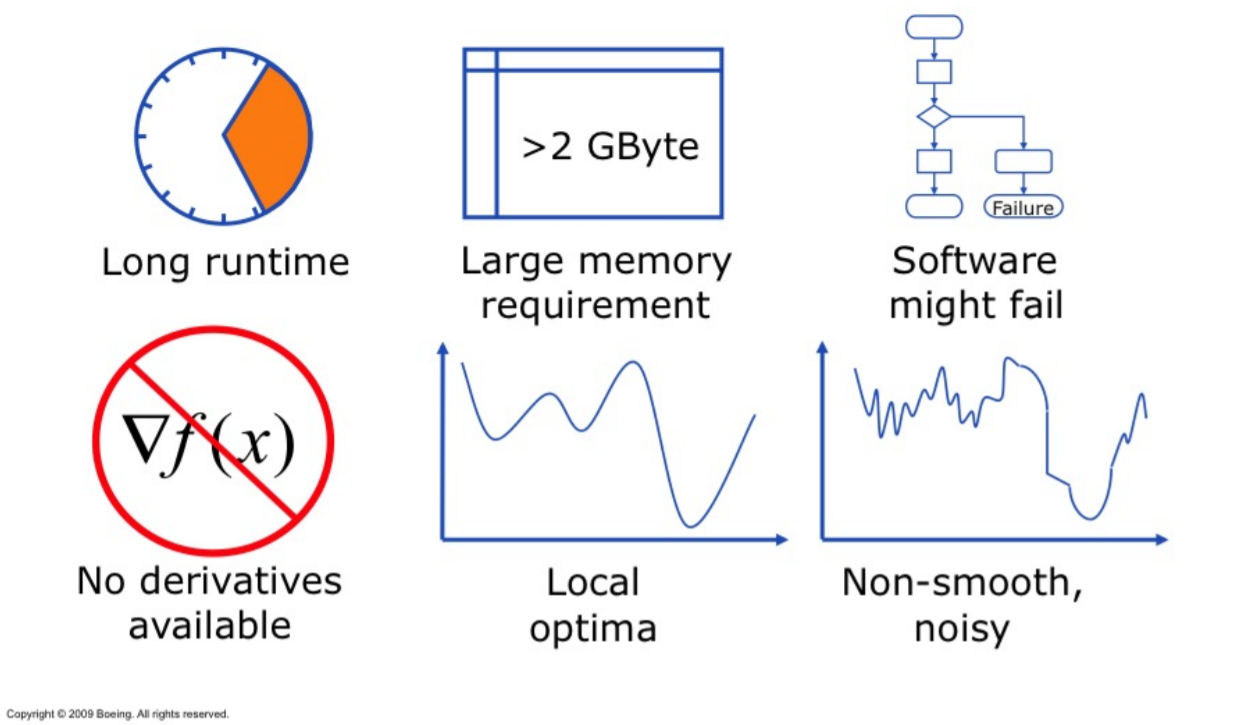
\includegraphics[width=\linewidth]{blackbox.png}
\end{frame}
\begin{frame}%5
\frametitle{Types d'algorithmes de DFO}
\textbf{Méthodes de région de confiance}
\smallskip
% Define block styles
%\tikzstyle{decision} = [diamond, draw, fill=blue!20, 
%text width=4.5em, text badly centered, node distance=3cm, inner sep=0pt]
\tikzstyle{block} = [rectangle, draw, fill=blue!20, 
text width=5em, text centered, rounded corners, minimum height=1em]
\tikzstyle{line} = [draw, -latex']
%
\begin{tikzpicture}[node distance = 6.3em, auto]
%% Place nodes
\node [block] (critic) {Criticalité};
\node [block, right of=critic] (step) {Calcul du pas};
\node [block, right of=step] (accept) {Acceptation du pas};
\node [block, right of=accept] (ameliore) {Amélioration du modèle};
\node [block, right of=ameliore] (udate) {Mise à jour de RDC};
%% Draw edges
\path [line] (critic) -- (step);
\path [line] (step) -- (accept);
\path [line] (accept) -- (ameliore);
\path [line] (ameliore) -- (udate);
\path [line] (udate) --++ (0cm,-1cm) -| (critic);
\end{tikzpicture}\\
\pause
\smallskip
\textbf{Méthodes de recherche directe}\\
\smallskip
% Define block styles
%\tikzstyle{decision} = [diamond, draw, fill=blue!20, 
%text width=4.5em, text badly centered, node distance=3cm, inner sep=0pt]
\tikzstyle{block} = [rectangle, draw, fill=blue!20, 
text width=6em, text centered, rounded corners, minimum height=1em]
\tikzstyle{line} = [draw, -latex']
%
\begin{minipage}[c]{0.45\textwidth}
\begin{tikzpicture}[node distance = 7.5em, auto]
%% Place nodes
\node [block] (sample) {Échantillonage};
\node [block, right of=sample] (udate) {Mise à jour de l'itéré courant};
%% Draw edges
\path [line] (sample) -- (udate);
\path [line] (udate) --++ (0cm,-1cm) -| (sample);
\end{tikzpicture}
\end{minipage}
\begin{minipage}[c]{0.45\textwidth}
\begin{itemize}
	\item[]\only<3-7>{Directionnelles (\MADS)}
	\item[]\only<4-7>{Simpliciales (Nelder-Mead)}
\end{itemize}
\end{minipage}\\
\smallskip
\only<5-7>{\textbf{Autres méthodes}}
\begin{itemize}
	\item[]\only<6-7>{Heuristiques (essaim de particules, recuit simulé)}
	\item[]\only<7>{Hybrides (filtrage implicite)}
\end{itemize}
\end{frame}
\begin{frame}%6
\frametitle{Problématique}
Notre but : réduire le nombre d'évaluations d'une boîte noire.
\pause
\medskip

Est-il toujours nécessaire d'évaluer tous les points déterminés lors des différentes étapes des méthodes?
\pause
\medskip

Si non, on étudiera alors l'impact de \textbf{la stratégie opportuniste}.

\pause
{\begin{block}{Stratégie opportuniste}
		La stratégie opportuniste désigne l'arrêt prématuré d'une étape d'un l'algorithme si les conditions pour passer à l'étape suivante sont déjà remplies.
\end{block}}
\pause
\medskip

Maintes fois  mentionnée et utilisée mais jamais étudiée en soi.
\end{frame}






\section{Recherche directe}
\tableofcontents[currentsection,currentsubsection,subsectionstyle=show/hide]
\subsection{Algorithmes}
\begin{frame}
\frametitle{Identification des méthodes}
\begin{exampleblock}{Question 1.}
Pour quelles méthodes est-ce valable?
\end{exampleblock}
Critère : les méthodes doivent posséder une liste de points.
\begin{itemize}
\item[]\only<2>{Région de confiance}\only<3->{{Région de confiance} {\color{red}\xmark}}
\item[]\only<3->{- Une seule évaluation de $f(x)$ pour une itération de l'algorithme}
\item[]\only<4>{Recherche directe simpliciales}\only<5->{Recherche directe simpliciales 
	{\color{red}\xmark}}
\item[]\only<5->{- Déja un arrêt prématuré et un ordre pré-déterminé}
\item[]\only<6>{Recherche directe directionnelles}\only<7->{\textbf{Recherche directe directionnelles} 
	{\checkmarkg}}
\item[]\only<7->{- Convergent vers un optimum indépendamment de l'arrêt prématuré.}
\item[]\only<8>{Recherche directe directionnelles hybrides}\only<9->{\textbf{Recherche directe directionnelles hybrides} \checkmarky}
\item[]\only<9->{- Convergent mais on peut altérer le bon fonctionnement.}
\item[]\only<10>{Heuristiques}\only<11->{Heuristiques \textbf{\large?}}
\item[]\only<11->{- Dépends de la forme de l'heuristique.}
\end{itemize}
\end{frame}

\begin{frame}%8
\frametitle{Cadre de travail en recherche directe}
\textbf{Méthodes de recherche directe directionelles} :
\begin{itemize}
	\pause
	\item Échantillonne $f(x)$ et $c(x)$ sur un ensemble fini de points.
	\pause
	\item Prends une action basée \underline{seulement sur ces valeurs}.
\end{itemize}
\pause
\setcounter{algorithm}{0}
\begin{minipage}{0.7\linewidth}
\begin{algorithm}[H]
	  \algsetup{linenosize=\tiny}
	\scriptsize
	\begin{algorithmic}[]
		\FOR{$k=1,2,\dots$}
		\STATE \textbf{Étape de recherche} : Calcule $f(x)$ à un ensemble de points $S^k$ issu de mécanismes heuristiques.
		\STATE Si succès, mise à jour de $x^k$
		\STATE
		\STATE \textbf{Étape de sonde} : Calcule $f(x)$ à un ensemble de points 
		\STATE $P^k:=\{x^k+\delta ^k d:d\in D\}$, où $D$ est un ensemble générateur positif. 
		\STATE Si succès, mise à jour de $x^k$
		\ENDFOR
	\end{algorithmic}
	\caption{Cadre de travail en recherche directe directionnelles}
	\label{alg:seq}
\end{algorithm}
\end{minipage}\\	
\textit{Remarque : on ne s'intéresse qu'aux étapes de sonde pour l'opportunisme.}
\end{frame}

\begin{frame}
\frametitle{Recherche par coordonnées (\CS)}
\begin{algorithm}[H]
\begin{algorithmic}[]
\FOR{$k=1,2,\dots$}
\STATE \textbf{Étape de sonde} : Calcule $f(x)$ à un ensemble de points $P^k:=\{x^k+\delta ^k d:d\in D_{\oplus}\}$, où $D_{\oplus} := \{\pm e_1,\pm e_2,\dots,\pm e_n\}$.
\STATE
\STATE Si $\exists~t$ tel que $f(t) < f(x^k)$, $t\in P^k$ : Succès
\STATE \tab mise à jour de $x^{k+1}\leftarrow t$ et $\delta^{k+1} \leftarrow \delta^k$.
\STATE
\STATE Sinon $\nexists~t$ tel que $f(t) < f(x^k)$, $t\in P^k$ : Échec
\STATE \tab mise à jour de $x^{k+1}\leftarrow x^k$ et $\delta^{k+1} \leftarrow \frac{\delta^k}{2}$.
\ENDFOR
\end{algorithmic}
\caption{Recherche par coordonnées}
\label{alg:cs}
\end{algorithm}
Si les évaluations sont séquentielles $\rightarrow$ On peut arrêter l'algorithme après un succès.
\end{frame}
%%%%%%%% exemple cs%%%%%%%%%%
\begin{frame}
	\frametitle{Recherche par coordonnées (\CS)}
	\only<1>{\begin{minipage}[t]{0.55\linewidth}
		\begin{figure}[H] %FIGURE  : MESH
			\begin{center}
				\begin{tikzpicture}
				% Flèches
				\draw [very thin,gray!50] (0,0) grid[step=0.5] (5,5);
				\draw [->,thick] (1.5,2.5)  -- (2.5,2.5) node [below,scale=0.65]{$f(t_1) = -1 $}; 
				\draw [->,thick] (1.5,2.5)  -- (0.5,2.5) node [below,scale=0.65]{$f(t_2) = 1 $}; 
				\draw [->,thick] (1.5,2.5) -- (1.5,3.5) node [above,scale=0.65]{$f(t_3) = -0.5 $};
				\draw [->,thick] (1.5,2.5) -- (1.5,1.5) node [below,scale=0.65]{$f(t_4) = 1.5 $};
				\draw (1.5,2.5) node [above right,scale=0.65]{$f(x^0) = 0$};
				\draw (1.5,2.5) node [scale=0.65] {$\bullet$};
				\end{tikzpicture}
			\end{center}
			\caption{\CS}
			\label{fig:CS1}
		\end{figure}
	\end{minipage}
\hfill
	\begin{minipage}[t]{0.40\linewidth}
		Ensemble des directions\\
		$D = \begin{bmatrix}
		1       & -1 & 0 & 0 \\
		0       & 0 & 1 & -1 \\
		\end{bmatrix}$\\
		Mise à jour, succès itération $k = {0}$\\
		$x^{1} \leftarrow x^0 + \delta^0 d_4$\\
		$\delta^{1} \leftarrow \delta^0$
	\end{minipage}}
		\only<2>{\begin{minipage}[t]{0.55\linewidth}
				\begin{figure}[H] %FIGURE  : MESH
					\begin{center}
						\begin{tikzpicture}
						% Flèches
						\draw [very thin,gray!50] (0,0) grid[step=0.5] (5,5);
						\draw [->,thick] (2.5,2.5)  -- (3.5,2.5) node [below right,scale=0.65]{$f(t_5) = -0.5 $}; 
						\draw [->,thick] (2.5,2.5)  -- (1.5,2.5) node [below,scale=0.65]{$f(t_6) = 0 $}; 
						\draw [->,thick] (2.5,2.5) -- (2.5,3.5) node [above,scale=0.65]{$f(t_7) = -0.8 $};
						\draw [->,thick] (2.5,2.5) -- (2.5,1.5) node [below,scale=0.65]{$f(t_8) = 2 $};
						\draw (2.5,2.5) node [above right,scale=0.65]{$f(x^1) = -1$};
						\draw (2.5,2.5) node [scale=0.65]{$\bullet$};
						\end{tikzpicture}
					\end{center}
					\caption{\CS}
					\label{fig:CS2}
				\end{figure}
			\end{minipage}
			\hfill
			\begin{minipage}[t]{0.40\linewidth}
				Ensemble des directions\\
				$D = \begin{bmatrix}
				1       & -1 & 0 & 0 \\
				0       & 0 & 1 & -1 \\
				\end{bmatrix}$\\
		Mise à jour, échec itération $k={1}$\\
		$x^{2} \leftarrow x^{1} $\\
		$\delta^{2} \leftarrow \frac{\delta^1}{2}$
		\end{minipage}}
		\only<3>{\begin{minipage}[t]{0.55\linewidth}
				\begin{figure}[H] %FIGURE  : MESH
					\begin{center}
						\begin{tikzpicture}
						% Flèches
						\draw [very thin,gray!50] (0,0) grid[step=0.5] (5,5);
						\draw [->,thick] (2.5,2.5)  -- (3,2.5) node [below right,scale=0.65]{$f(t_9)$}; 
						\draw [->,thick] (2.5,2.5)  -- (2,2.5) node [below,scale=0.65]{$f(t_{10})$}; 
						\draw [->,thick] (2.5,2.5) -- (2.5,3) node [above,scale=0.65]{$f(t_{11})$};
						\draw [->,thick] (2.5,2.5) -- (2.5,2) node [below,scale=0.65]{$f(t_{12})$};
						\draw (2.5,2.5) node [above right,scale=0.65]{$f(x^2) = -1$};
						\draw (2.5,2.5) node [scale=0.65]{$\bullet$};
						\end{tikzpicture}
					\end{center}
					\caption{\CS}
					\label{fig:CS3}
				\end{figure}
			\end{minipage}
			\hfill
			\begin{minipage}[t]{0.40\linewidth}
				~
		\end{minipage}}
\end{frame}
%%%%%%%%%%% ALGO GPS
\begin{frame}
\frametitle{Recherche par motifs généralisée (\GPS)}
\begin{algorithm}[H]
\begin{algorithmic}[]
\FOR{$k=1,2,\dots$}
\STATE avec $\tau \in \{0,1\}$.
\STATE \textbf{Étape de sonde} : Calcule $f(x)$ à un ensemble de points $P^k:=\{x^k+\delta ^k d:d\in D\}$, où {\color{red}$D$ est un ensemble générateur positif.}
\STATE
\STATE Si $\exists~t$ tel que $f(t) < f(x^k)$, $t\in P^k$ : Succès
\STATE \tab mise à jour de $x^{k+1}\leftarrow t$ et $\delta^{k+1} \leftarrow {\color{red}\tau^{-1}}\delta^k$.
\STATE
\STATE Sinon $\nexists~t$ tel que $f(t) < f(x^k)$, $t\in P^k$ : Échec
\STATE \tab mise à jour de $x^{k+1}\leftarrow x^k$ et $\delta^{k+1} \leftarrow {\color{red}\tau}\delta^k$.
\ENDFOR
\end{algorithmic}
\caption{Recherche par motifs généralisée}
\label{alg:gps}
\end{algorithm}
\end{frame}
%%%%%%%%% exemple gps
\begin{frame}
\frametitle{Recherche par motifs généralisée (\GPS)}
\only<1>{\begin{minipage}[t]{0.55\linewidth}
		\begin{figure}[H] %FIGURE  : MESH
			\begin{center}
				\begin{tikzpicture}
				% Flèches
				\draw [very thin,gray!50] (0,0) grid[step=0.5] (5.5,5.5);
				\draw [->,thick] (1.5,2.5) -- (2.5,3.5) node [above,scale=0.65]{$f(t_1) = -0.9 $};
				\draw [->,thick] (1.5,2.5)  -- (0.5,2.5) node [below,scale=0.65]{$f(t_2) = 1 $}; 
				\draw [->,thick] (1.5,2.5)  -- (1.5,1.5) node [below,scale=0.65]{$f(t_3) = 2 $};
				\draw (1.5,2.5) node [right,scale=0.65]{$f(x^0) = 0$};
				\draw (1.5,2.5) node [scale=0.65] {$\bullet$};
				\end{tikzpicture}
			\end{center}
			\caption{\GPS}
			\label{fig:GPS1}
		\end{figure}
	\end{minipage}
	\hfill
	\begin{minipage}[t]{0.40\linewidth}
		Paramètres\\
		$\tau = \frac{2}{3}$,  \\
		$D = \begin{bmatrix}
		1       & -1 & 1 \\
		0       & 0 & 1 \\
		\end{bmatrix}$\\\\
		Mise à jour, succès itération $k={0}$\\
		$x^{1} \leftarrow x^0 + \delta^0 d_3$\\
		$\delta^{1} \leftarrow \frac{3}{2}\delta^0$
\end{minipage}}
\only<2>{\begin{minipage}[t]{0.55\linewidth}
		\begin{figure}[H] %FIGURE  : MESH
			\begin{center}
				\begin{tikzpicture}
				% Flèches
				\draw [very thin,gray!50] (0,0) grid[step=0.5] (5.5,5.5);
				\draw [->,thick] (2.5,3.5) -- (4,5) node [below right,scale=0.65]{$f(t_4) = 3 $};
				\draw [->,thick] (2.5,3.5)  -- (1,3.5) node [below,scale=0.65]{$f(t_5) = 0 $}; 
				\draw [->,thick] (2.5,3.5)  -- (2.5,2) node [below,scale=0.65]{$f(t_6) = 0.6 $};
				\draw (2.5,3.5) node [right,scale=0.65]{$f(x^1) = -0.9$};
				\draw (2.5,3.5) node [scale=0.65] {$\bullet$};
				\end{tikzpicture}
			\end{center}
			\caption{\GPS}
			\label{fig:GPS2}
		\end{figure}
	\end{minipage}
	\hfill
	\begin{minipage}[t]{0.40\linewidth}
			Paramètres\\
	$\tau = \frac{2}{3}$,  \\
	$D = \begin{bmatrix}
	1       & -1 & 1 \\
	0       & 0 & 1 \\
	\end{bmatrix}$\\\\
		Mise à jour, échec itération $k={1}$\\
		$x^{2} \leftarrow x^1$\\
		$\delta^{2} \leftarrow \frac{2}{3}\delta^1$
\end{minipage}}
\only<3>{\begin{minipage}[t]{0.55\linewidth}
		\begin{figure}[H] %FIGURE  : MESH
			\begin{center}
				\begin{tikzpicture}
				% Flèches
				\draw [very thin,gray!50] (0,0) grid[step=0.5] (5.5,5.5);
				\draw [->,thick] (2.5,3.5) -- (3.5,4.5) node [above,scale=0.65]{$f(t_7)$};
				\draw [->,thick] (2.5,3.5)  -- (1.5,3.5) node [below,scale=0.65]{$f(t_8)$}; 
				\draw [->,thick] (2.5,3.5)  -- (2.5,2.5) node [below,scale=0.65]{$f(t_9)$};
				\draw (2.5,3.5) node [right,scale=0.65]{$f(x^2) = -0.9$};
				\draw (2.5,3.5) node [scale=0.65] {$\bullet$};
				\end{tikzpicture}
			\end{center}
			\caption{\GPS}
			\label{fig:GPS3}
		\end{figure}
	\end{minipage}
	\hfill
	\begin{minipage}[t]{0.40\linewidth}
\end{minipage}}
\end{frame}
%%%%%%%%%%%%%
\begin{frame}
\frametitle{Recherche par ensemble générateurs (\GSS)}
\begin{algorithm}[H]
\begin{algorithmic}[]
\FOR{$k=1,2,\dots$}
\STATE avec $\tau \in \{0,1\}$, $\phi > 0$.
\STATE \textbf{Étape de sonde} : Calcule $f(x)$ à un ensemble de points 
\STATE $P^k:=\{x^k+\delta ^k d:d\in D\}$, où {\color{blue}$D$ est un ensemble générateur 
\STATE respectant certaines conditions}.
\STATE
\STATE Si $\exists~t$ tel que $f(t) < f(x^k){\color{blue}-\rho(\delta^k)}$, $t\in P^k$ : Succès
\STATE \tab mise à jour de $x^{k+1}\leftarrow t$ et $\delta^{k+1} \leftarrow {\color{blue}\phi}\delta^k$.
\STATE
\STATE Sinon $\nexists~t$ tel que $f(t) < f(x^k){\color{blue}-\rho(\delta^k)}$, $t\in P^k$ : Échec
\STATE \tab mise à jour de $x^{k+1}\leftarrow x^k$ et $\delta^{k+1} \leftarrow {\color{red}\tau}\delta^k$.
\ENDFOR
\end{algorithmic}
\caption{Recherche par ensemble générateurs}
\label{alg:gss}
\end{algorithm}
L'analyse de converge est basée sur \textbf{la condition de décroissance minimale}.
\end{frame}
%%%%%%%%%%%%%%%%%% exemple GSS
\begin{frame}
\frametitle{Recherche par ensembles générateurs (\GSS)}
\only<1>{\begin{minipage}[t]{0.55\linewidth}
		\begin{figure}[H] %FIGURE  : MESH
			\begin{center}
				\begin{tikzpicture}
				% Flèches
				\draw [very thin,white!50] (0,0) grid[step=0.5] (5.5,5.5);
				\draw [->,thick] (1.5,2.5) -- (2.5,3.5) node [above,scale=0.65]{$f(t_1) = -0.9 $};
				\draw [->,thick] (1.5,2.5)  -- (0.5,2.5) node [below,scale=0.65]{$f(t_2) = 1 $}; 
				\draw [->,thick] (1.5,2.5)  -- (1.5,1.5) node [below,scale=0.65]{$f(t_3) = 2 $};
				\draw (1.5,2.5) node [right,scale=0.65]{$f(x^0) = 0$};
				\draw (1.5,2.5) node [scale=0.65] {$\bullet$};
				\end{tikzpicture}
			\end{center}
			\caption{\GSS}
			\label{fig:GSS1}
		\end{figure}
	\end{minipage}
	\hfill
	\begin{minipage}[t]{0.40\linewidth}
		Paramètres\\
		$\phi = \frac{3}{2}$, 
		$\tau = \frac{1}{2}$, \\
		 $ D = \begin{bmatrix}
		1       & -1 & 1 \\
		0       & 0 & 1 \\
		\end{bmatrix}$\\\\
		Mise à jour, succès itération $k={0}$\\\\
		$\color{blue} f(t_1) < f(x^1)-\rho(\delta^1)$\\
		$x^{1} \leftarrow x^0 + \delta^0 d_3$\\
		$\delta^{1} \leftarrow \frac{3}{2}\delta^0$
\end{minipage}}
\only<2>{\begin{minipage}[t]{0.55\linewidth}
		\begin{figure}[H] %FIGURE  : MESH
			\begin{center}
				\begin{tikzpicture}
				% Flèches
				\draw [very thin,white!50] (0,0) grid[step=0.5] (5.5,5.5);
				\draw [->,thick] (2.5,3.5) -- (4,5) node [below right,scale=0.65]{$f(t_4) = 3 $};
				\draw [->,thick] (2.5,3.5)  -- (1,3.5) node [below,scale=0.65]{$f(t_5) = 0 $}; 
				\draw [->,thick] (2.5,3.5)  -- (2.5,2) node [below,scale=0.65]{$f(t_6) = -0.91 $};
				\draw (2.5,3.5) node [right,scale=0.65]{$f(x^1) = -0.9$};
				\draw (2.5,3.5) node [scale=0.65] {$\bullet$};
				\end{tikzpicture}
			\end{center}
			\caption{\GSS}
			\label{fig:GSS2}
		\end{figure}
	\end{minipage}
	\hfill
	\begin{minipage}[t]{0.40\linewidth}
			Paramètres\\
		$\phi = \frac{3}{2}$, 
		$\tau = \frac{1}{2}$, \\
		$ D = \begin{bmatrix}
		1       & -1 & 1 \\
		0       & 0 & 1 \\
		\end{bmatrix}$\\\\
		Mise à jour, échec itération $k={1}$\\\\
		$\color{red} f(t_6) > f(x^1)-\rho(\delta^1)$\\
		$x^{2} \leftarrow x^1$\\
		$\delta^{2} \leftarrow \frac{1}{2}\delta^1$
\end{minipage}}
\only<3>{\begin{minipage}[t]{0.55\linewidth}
		\begin{figure}[H] %FIGURE  : MESH
			\begin{center}
				\begin{tikzpicture}
				% Flèches
				\draw [very thin,white!50] (0,0) grid[step=0.5] (5.5,5.5);
				\draw [->,thick] (2.5,3.5) -- (3.25,4.25) node [above,scale=0.65]{$f(t_7)$};
				\draw [->,thick] (2.5,3.5)  -- (1.75,3.5) node [below,scale=0.65]{$f(t_8)$}; 
				\draw [->,thick] (2.5,3.5)  -- (2.5,2.75) node [below,scale=0.65]{$f(t_9)$};
				\draw (2.5,3.5) node [right,scale=0.65]{$f(x^2) = -0.9$};
				\draw (2.5,3.5) node [scale=0.65] {$\bullet$};
				\end{tikzpicture}
			\end{center}
			\caption{\GSS}
			\label{fig:GSS3}
		\end{figure}
	\end{minipage}
	\hfill
	\begin{minipage}[t]{0.40\linewidth}
\end{minipage}}
\end{frame}
%%%%%%%%%%% MADS algo
\begin{frame}
\frametitle{Recherche par treillis adaptatifs (\MADS)}
\begin{algorithm}[H]
\begin{algorithmic}[]
\FOR{$k=1,2,\dots$}
\STATE avec $\tau \in \{0,1\}$.
\STATE {\color{red}Mise à jour : $\delta^k \leftarrow \min(\Delta^k,(\Delta^k)^2)$}
\STATE \textbf{Étape de sonde} : Calcule $f(x)$ à un ensemble de points 
\STATE $P^k:=\{x^k+\delta ^k d:d\in D\}$, où {\color{red}$D\subset F^k$,
\STATE avec $F^k$ le cadre de demi côté $\Delta^k$.}
\STATE
\STATE Si $\exists~t$ tel que $f(t) < f(x^k)$, $t\in P^k$ : Succès
\STATE \tab mise à jour de $x^{k+1}\leftarrow t$ et ${\color{red}\Delta^{k+1}} \leftarrow {\color{red}\tau^{-1}\Delta^k}$.
\STATE
\STATE Sinon $\nexists~t$ tel que $f(t) < f(x^k)$, $t\in P^k$ : Échec
\STATE \tab mise à jour de $x^{k+1}\leftarrow x^k$ et ${\color{red}\Delta^{k+1}} \leftarrow {\color{red}\tau\Delta^k}$.
\ENDFOR
\end{algorithmic}
\caption{Recherche par treillis adaptatifs}
\label{alg:mads}
\end{algorithm}
\end{frame}
%%%%%%% MADS EXEMPLE
\begin{frame}
\frametitle{Recherche par motifs généralisée (\MADS)}
\only<1>{\begin{minipage}[t]{0.55\linewidth}
		\begin{figure}[H] %FIGURE  : MESH
			\begin{center}
				\begin{tikzpicture}
				% Flèches
				\draw [very thin,gray!50] (0,0) grid[step=0.25] (5.5,5.5);
				\draw [very thick] (0.5,1.5) rectangle (2.5,3.5);
				\draw [->,thick] (1.5,2.5) -- (2.5,3.5) node [above,scale=0.65]{$f(t_1) = -0.9 $};
				\draw [->,thick] (1.5,2.5)  -- (0.5,2.5) node [below,scale=0.65]{$f(t_2) = 1 $}; 
				\draw [->,thick] (1.5,2.5)  -- (1.5,1.5) node [below,scale=0.65]{$f(t_3) = 2 $};
				\draw (1.5,2.5) node [right,scale=0.65]{$f(x^0) = 0$};
				\draw (1.5,2.5) node [scale=0.65] {$\bullet$};
				\end{tikzpicture}
			\end{center}
			\caption{\MADS}
			\label{fig:MADS1}
		\end{figure}
	\end{minipage}
	\hfill
	\begin{minipage}[t]{0.40\linewidth}
		Paramètres\\
		$\tau = \frac{2}{3}$,  \\
		$D = \begin{bmatrix}
		1       & -1 & 1 \\
		0       & 0 & 1 \\
		\end{bmatrix}$\\\\
		Mise à jour, succès itération $k={0}$\\
		$x^{1} \leftarrow t_1$\\
		$\Delta^{1} \leftarrow \frac{3}{2}\Delta^0$\\
\end{minipage}}
\only<2>{\begin{minipage}[t]{0.55\linewidth}
		\begin{figure}[H] %FIGURE  : MESH
			\begin{center}
				\begin{tikzpicture}
				% Flèches
				\draw [very thin,gray!50] (0,0) grid[step=0.5] (5.5,5.5);
				\draw [very thick] (1,2) rectangle (4,5);
				\draw [->,thick] (2.5,3.5) -- (1,3.5) node [below right,scale=0.65]{$f(t_4) = 3 $};
				\draw [->,thick] (2.5,3.5)  -- (2.5,5) node [below,scale=0.65]{$f(t_5) = 0 $}; 
				\draw [->,thick] (2.5,3.5)  -- (4,2) node [below,scale=0.65]{$f(t_6) = 0.6 $};
				\draw (2.5,3.5) node [right,scale=0.65]{$f(x^1) = -0.9$};
				\draw (2.5,3.5) node [scale=0.65] {$\bullet$};
				\end{tikzpicture}
			\end{center}
			\caption{\MADS}
			\label{fig:MADS2}
		\end{figure}
	\end{minipage}
	\hfill
	\begin{minipage}[t]{0.40\linewidth}
		Paramètres\\
		$\tau = \frac{2}{3}$,  \\
		$D = \begin{bmatrix}
		1       & -1 & 1 \\
		0       & 0 & 1 \\
		\end{bmatrix}$\\\\
		Mise à jour, échec itération $k={1}$\\
		$x^{2} \leftarrow x^1$\\
		$\Delta^{2} \leftarrow \frac{2}{3}\Delta^1$
\end{minipage}}
\only<3>{\begin{minipage}[t]{0.55\linewidth}
		\begin{figure}[H] %FIGURE  : MESH
			\begin{center}
				\begin{tikzpicture}
				% Flèches
				\draw [very thin,gray!50] (0,0) grid[step=0.25] (5.5,5.5);
				\draw [very thick] (1.5,2.5) rectangle (3.5,4.5);
				\draw [->,thick] (2.5,3.5) -- (3.5,3.25) node [right,scale=0.65]{$f(t_7)$};
				\draw [->,thick] (2.5,3.5)  -- (1.75,4.5) node [above,scale=0.65]{$f(t_8)$}; 
				\draw [->,thick] (2.5,3.5)  -- (1.5,2.75) node [below left,scale=0.65]{$f(t_9)$};
				\draw (2.5,3.5) node [above right,scale=0.65]{$f(x^2)$};
				\draw (2.5,3.5) node [scale=0.65] {$\bullet$};
				\end{tikzpicture}
			\end{center}
			\caption{\MADS}
			\label{fig:MADS3}
		\end{figure}
	\end{minipage}
	\hfill
	\begin{minipage}[t]{0.40\linewidth}
\end{minipage}}
\end{frame}
%%%%%% IMFIL ALGO
\begin{frame}
\begin{algorithm}[H]
\begin{algorithmic}[]
\FOR{$k=1,2,\dots$}
\STATE \textbf{Étape de sonde} : Calcule $f(x)$ à un ensemble de points
\STATE $P^k:=\{x^k+\delta ^k d:d\in D_{\oplus}\}$, où $D_{\oplus} := \{\pm e_1,\pm e_2,\dots,\pm e_n\}$.
\STATE
\STATE Si $\exists~t$ tel que $f(t) < f(x^k)$, $t\in P^k$ : Succès
\STATE {\color{red}Effectuer une recherche linéaire avec $\nabla_s f(x^k)$.}
\STATE \tab mise à jour de $x^{k+1}\leftarrow t$ et $\delta^{k+1} \leftarrow \delta^k$.
\STATE
\STATE Sinon $\nexists~t$ tel que $f(t) < f(x^k)$, $t\in P^k$ : Échec
\STATE \tab mise à jour de $x^{k+1}\leftarrow x^k$ et $\delta^{k+1} \leftarrow \frac{\delta^k}{2}$.
\ENDFOR
\end{algorithmic}
\caption{Filtrage implicite}
\label{alg:imfil}
\end{algorithm}
\frametitle{Filtrage implicite (\IMFIL)}
\end{frame}
%%%%%%%%% EXEMPLE IMFIL
\begin{frame}
\frametitle{Filtrage implicite (\IMFIL)}
\only<1>{\begin{minipage}[t]{0.55\linewidth}
		\begin{figure}[H] %FIGURE  : MESH
			\begin{center}
				\begin{tikzpicture}
				% Flèches
				\draw [very thin,gray!50] (0,0) grid[step=0.5] (5,5);
				\draw [->,thick] (1.5,2.5)  -- (2.5,2.5) node [below,scale=0.65]{$f(t_1) = -1 $}; 
				\draw [->,thick] (1.5,2.5)  -- (0.5,2.5) node [below,scale=0.65]{$f(t_2) = 1 $}; 
				\draw [->,thick] (1.5,2.5) -- (1.5,3.5) node [above,scale=0.65]{$f(t_3) = -0.5 $};
				\draw [->,thick] (1.5,2.5) -- (1.5,1.5) node [below,scale=0.65]{$f(t_4) = 1.5 $};
				\draw (1.5,2.5) node [above right,scale=0.65]{$f(x^0) = 0$};
				\draw (1.5,2.5) node [scale=0.65] {$\bullet$};
				\end{tikzpicture}
			\end{center}
			\caption{\IMFIL}
			\label{fig:imfil1}
		\end{figure}
	\end{minipage}
	\hfill
	\begin{minipage}[t]{0.40\linewidth}
		Ensemble des directions\\
		$D = \begin{bmatrix}
		1       & -1 & 0 & 0 \\
		0       & 0 & 1 & -1 \\
		\end{bmatrix}$\\\\
		Calcul de $\nabla_s f(x^0)$\\
		Recherche linéaire $\rightarrow t_5$
\end{minipage}}
\only<2>{\begin{minipage}[t]{0.55\linewidth}
		\begin{figure}[H] %FIGURE  : MESH
			\begin{center}
				\begin{tikzpicture}
				% Flèches
				\draw [very thin,gray!50] (0,0) grid[step=0.5] (5,5);
				\draw [->,thick] (1.5,2.5)  -- (2.5,2.5) node [below,scale=0.65]{$f(t_1) = -1 $}; 
				\draw [->,thick] (1.5,2.5)  -- (0.5,2.5) node [below,scale=0.65]{$f(t_2) = 1 $}; 
				\draw [->,thick] (1.5,2.5) -- (1.5,3.5) node [above,scale=0.65]{$f(t_3) = -0.5 $};
				\draw [->,thick] (1.5,2.5) -- (1.5,1.5) node [below,scale=0.65]{$f(t_4) = 1.5 $};
				\draw [->,thick,red] (1.5,2.5) -- (3,4) node [above, scale = 0.65]{$-\nabla_sf(x^0)$};
				\draw [red] (3,4) node [below right,scale=0.65]{$f(t_5) = -1.5$};
				\draw (1.5,2.5) node [above right,scale=0.65]{$f(x^0) = 0$};
				\draw (1.5,2.5) node [scale=0.65] {$\bullet$};
				\end{tikzpicture}
			\end{center}
			\caption{\IMFIL}
			\label{fig:imfil2}
		\end{figure}
	\end{minipage}
	\hfill
	\begin{minipage}[t]{0.40\linewidth}
		Ensemble des directions\\
		$D = \begin{bmatrix}
		1       & -1 & 0 & 0 \\
		0       & 0 & 1 & -1 \\
		\end{bmatrix}$\\\\
		$-\nabla_s f(x^0) = \begin{bmatrix}
		1\\
		1
		\end{bmatrix}$\\
		Mise à jour, succès itération $k = {0}$\\
		$x^{1} \leftarrow x^0 -\beta^1 \nabla_s f(x^0)$\\
		$\delta^{1} \leftarrow \delta^0$
\end{minipage}}
\only<3>{\begin{minipage}[t]{0.55\linewidth}
		\begin{figure}[H] %FIGURE  : MESH
			\begin{center}
				\begin{tikzpicture}
				% Flèches
				\draw [very thin,gray!50] (0,0) grid[step=0.5] (5,5);
				\draw [->,thick] (3,4)  -- (4,4) node [below,scale=0.65]{$f(t_6)$}; 
				\draw [->,thick] (3,4)  -- (3,5) node [below right,scale=0.65]{$f(t_7)$}; 
				\draw [->,thick] (3,4) -- (2,4) node [above,scale=0.65]{$f(t_8)$};
				\draw [->,thick] (3,4) -- (3,3) node [below,scale=0.65]{$f(t_9)$};
				\draw (3,4) node [above right,scale=0.65]{$f(x^1) = -1.5$};
				\draw (3,4) node [scale=0.65] {$\bullet$};
				\end{tikzpicture}
			\end{center}
			\caption{\IMFIL}
			\label{fig:imfil3}
		\end{figure}
	\end{minipage}
	\hfill
	\begin{minipage}[t]{0.40\linewidth}
~
\end{minipage}}
\end{frame}
%%%%%%%%%%%%%%%%%%%
%%%%%%%%%%%%%%5555
\section{Opportunisme et ordonnancement}
\tableofcontents[currentsection,currentsubsection,subsectionstyle=show/hide]
\subsection{Opportunisme}
\begin{frame}
\frametitle{Définitions}
\begin{exampleblock}{Question 2.}
Quand doit-on arrêter la sonde?
\end{exampleblock}
\pause
\bigskip

\pause
\bigskip

{\begin{block}{Sonde complète}
Désigne l'évaluation de la fonction objectif à tous les points de l'étape de sonde.
\end{block}}
\pause
\bigskip

\begin{block}{Stratégie opportuniste simple}
	Désigne l'arrêt prématuré de la sonde à \textbf{l'obtention d'un point} satisfaisant le critère de succès. 
\end{block}
\end{frame}
%%%%%% Slide exemple opportunisme
\begin{frame}%6
\frametitle{Exemple de sonde opportuniste}
Supposons \CS~ pour résoudre $f:\R^3\mapsto \R$, avec $x^k = (2,2,2)$, $f(x^k) = 0$.\\
\bigskip
\begin{minipage}[t]{0.49\linewidth}
	{\footnotesize Sonde non-opportuniste
		
		$P^k := $
		\begin{itemize}
			\item[]\only<1>{$t_1 = (1,2,2)$}\only<2->{$t_1 = (1,2,2),~f(t_1) = 2 ${\color{red}\xmark}}
			\item[]\only<1-2>{$t_2 = (2,1,2)$}\only<3->{$t_2 = (2,1,2),~f(t_2) = 1${\color{red}\xmark}}
			\item[]\only<1-3>{$t_3 = (2,2,1)$}\only<4->{$t_3 = (2,2,1),~f(t_3) = -1$\checkmarkg}
			\item[]\only<1-4>{$t_4 = (2,2,3)$}\only<5->{$t_4 = (2,2,3),~f(t_4) = 5${\color{red}\xmark}}
			\item[]\only<1-5>{$t_5 = (2,3,2)$}\only<6->{$t_5 = (2,3,2),~f(t_5) = -1.5$\checkmarkg}
			\item[]\only<1-6>{$t_6 = (3,2,2)$}\only<7->{$t_6 = (3,2,1),~f(t_6) = 6${\color{red}\xmark}}
		\end{itemize}
	}
\end{minipage}
\begin{minipage}[t]{0.49\linewidth}
	{\footnotesize Sonde opportuniste
		
		$P^k := $
		\begin{itemize}
			\item[]\only<1-7>{$t_1 = (1,2,2)$}\only<8->{$t_1 = (1,2,2),~f(t_1) = 2 ${\color{red}\xmark}}
			\item[]\only<1-8>{$t_2 = (2,1,2)$}\only<9->{$t_2 = (2,1,2),~f(t_2) = 1${\color{red}\xmark}}
			\item[]\only<1-9>{$t_3 = (2,2,1)$}\only<10->{$t_3 = (2,2,1),~f(t_3) = -1$\checkmarkg}
			\item[]\only<1-9>{$t_4 = (2,2,3)$}\only<10->{\sout{$t_4 = (2,2,3)$}}
			\item[]\only<1-9>{$t_5 = (2,3,2)$}\only<10->{\sout{$t_5 = (2,3,2)$}}
			\item[]\only<1-9>{$t_6 = (3,2,2)$}\only<10->{\sout{$t_6 = (3,2,1)$}}
		\end{itemize}
	}
\end{minipage}
\end{frame}
%%%%%%%%55555
\begin{frame}
\frametitle{Différentes stratégies opportunistes}

\begin{block}{Stratégie opportuniste au $p$\textsuperscript{ème} succès}
Arrêt de la sonde après \textbf{l'obtention de $p$ points} satisfaisant le critère de succès.\end{block}
\pause
\medskip

{\begin{block}{Stratégie opportuniste avec au minimum $q$ évaluations}
Arrêt de la sonde \textbf{après $q$ évaluations} si un point satisfaisant le critère de succès est évalué. \end{block}}
\end{frame}

\begin{frame}
\frametitle{Définitions}
\begin{exampleblock}{Question 3.}
Comment doit-on ordonner les points de $P^k$?
\end{exampleblock}
\pause
\bigskip

{\begin{block}{Stratégie d'ordonnancement}
Stratégie guidant la permutation des points de l'ensemble $P^k$.
\end{block}}
\end{frame}

\begin{frame}
\frametitle{Stratégies d’ordonnancement}
\begin{enumerate}
\item\only<1->{\textbf{Lexicographique}}
\pause
\item[]\only<2->{Ordonnés comme dans un dictionnaire.}
\pause
\item\only<3->{\textbf{Aléatoire}}
\pause
\item\only<4->{\textbf{Direction du dernier succès}}
\pause
\item[]\only<5->{Ordonnés selon l'angle avec la direction du dernier succès.}
\pause
\item\only<6->{\textbf{Guidé par modèle quadratique}}
\pause
\item[]\only<7->{$A\prec B$ si $\tilde{f}(A) < \tilde{f}(B)$}
\item[]\only<8->{$\tilde{f}$ une fonction substitut quadratique de $f$.}
\end{enumerate}
\end{frame}

\begin{frame}
\frametitle{Stratégies de comparaison}
Déterminer la \underline{meilleure} amélioration possible avec l'ordonnancement :
\pause
\begin{itemize}
\item[\mynum{5}]\only<2->{\textbf{Omnisciente}}
\pause
\item[]\only<3->{$A \prec B$ si $f(A)<f(B)$}
\end{itemize}
\pause
\bigskip
\only<4->{Déterminer le \underline{pire} ordonnancement possible : }
\pause
\begin{enumerate}
\item[\mynum{6}]\only<5->{\textbf{Inverse-Omnisciente}}
\pause
\item[]\only<6->{$A \prec B$ si $f(A)>f(B)$}
\end{enumerate}
\bigskip
\pause

\begin{center}
{\color{red} \Large Impossible à appliquer en pratique}
\end{center}
\end{frame}

\section{Tests numériques}
\tableofcontents[currentsection,currentsubsection,subsectionstyle=show/hide]
\subsection{Résultats numériques}
\begin{frame}
\frametitle{Problèmes tests}
\begin{enumerate}
\item\only<1->{212 instances de problèmes issus de \cite{MoWi2009}}
\pause
\item\only<2->{18 problèmes contraints issus de \cite{AuTr17}}
\pause
\item[]\only<3->{$x^0$ irréalisable}
\pause
\item\only<4->{1 Boîte noire, STYRENE, issue de \cite{AuBeLe08}}
\pause
\item[]\only<5->{$f:R^8\mapsto R$, $c:R^8\mapsto R^{11}$, 4 contraintes binaire, 7 contraintes relaxables}
\end{enumerate}
\pause
\begin{center}
\begin{figure}
	\centering
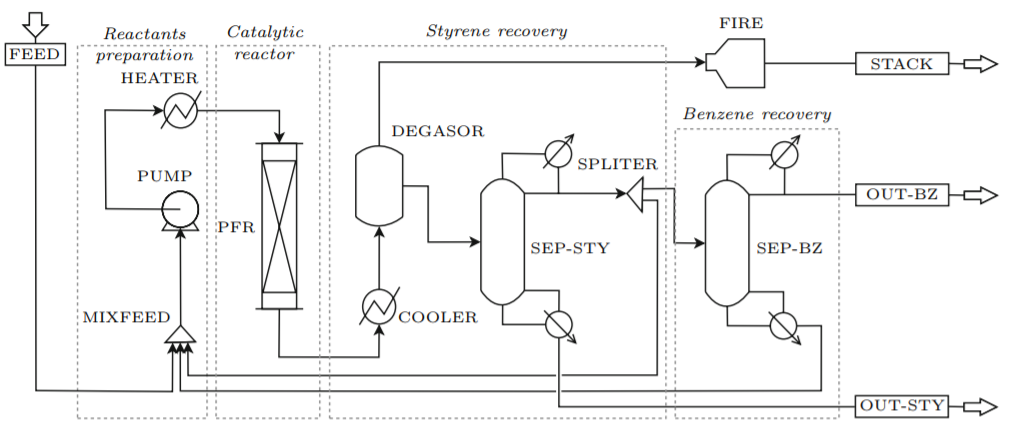
\includegraphics[width=7cm]{StyreneFlow.PNG}
\caption{Organigramme de la production de Styrène, issu de \cite{AuBeLe08}}
\end{figure}
\end{center}
\end{frame}

\begin{frame}
\frametitle{Comparaison des stratégies opportunistes}
\noindent
\begin{center}
\begin{figure}
\vspace{-1em}
\begin{minipage}[t]{0.45\linewidth}
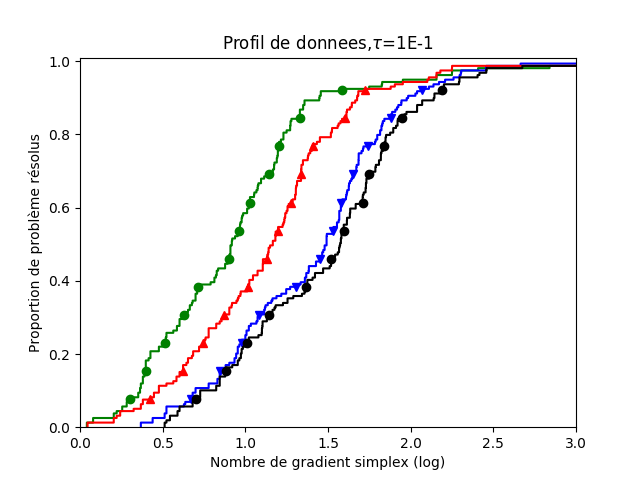
\includegraphics[width=\linewidth]{coppcomp.png}
\end{minipage}
\hfill%
\begin{minipage}[t]{0.45\linewidth}
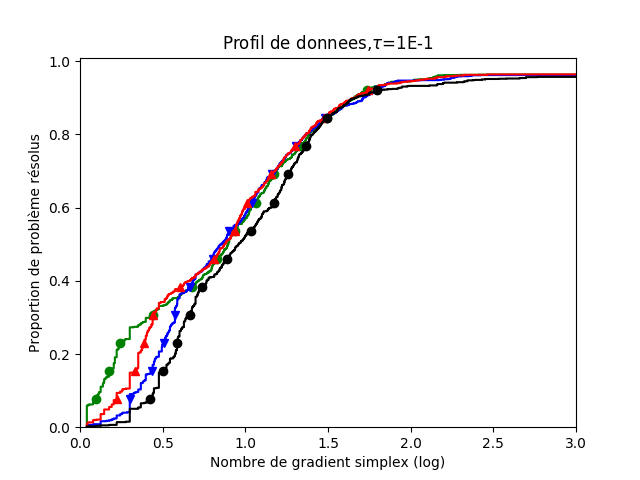
\includegraphics[width=\linewidth]{moppcomp.png}
\end{minipage}

\includegraphics[width=\linewidth]{Legende_comp.png}
\vspace{-1.5em}
\caption{À gauche : \CS~sur Moré-Wild, à droite \MADS~sur Moré-Wild}
\vspace{-1.3em}
\end{figure}
\end{center}
\begin{minipage}[t]{0.5\linewidth}
\begin{enumerate}
\pause
\item Ordonnancement simple plus efficace.
\pause
\item Autres stratégies $\rightarrow$ Sonde complète.
\end{enumerate}
\end{minipage}%
\hfill%
\begin{minipage}[t]{0.5\linewidth}
\begin{enumerate}
\pause
\item[\mynum{3}] Impact moins important sur \MADS.
\end{enumerate}
\end{minipage}
\end{frame}
%%%%%%%%%%%%%%%%%%%%%%%%%%%%%%%%%%%%%%%%%%%%%%%%%%55
%%%%%%%%%%%%%%%%%%%%%%%%%%%%%%%%%%%%%%%%%%%%%%%%%%%55
\begin{frame}
\frametitle{Comparaison des stratégies d'ordonnancement}
\noindent
	\begin{center}
		\begin{figure}
		\vspace{-1em}
			\begin{minipage}[t]{0.5\linewidth}
				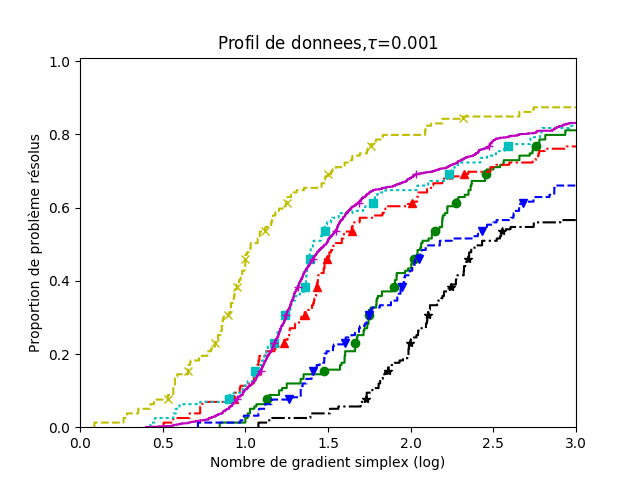
\includegraphics[width=\linewidth]{cog.png}
			\end{minipage}\\
		
\includegraphics[width=\linewidth]{legende_mw.png}
		\vspace{-1em}
		\caption{\CS~sur Moré-Wild}
		\vspace{-1.3em}
		\end{figure}
	\end{center}
%%%%%%%%%%%%%%%%%%%%%
%\begin{minipage}[t]{0.5\linewidth}
%\begin{enumerate}
%\pause
%\item Grand impact de l'ordonnancement sur \CS.
%\end{enumerate}
%\end{minipage}%
%\hfill%
%\begin{minipage}[t]{0.5\linewidth}
%\begin{enumerate}
%\pause
%\item[\mynum{2}] Hiérarchie des stratégies observable.
%%\pause
%%\item[\mynum{3}] Impact moins important sur \MADS.
%%\pause
%%\item[\mynum{4}] Classement différent sur \CS~ et \MADS.
%\end{enumerate}
%\end{minipage}
\end{frame}
%%%%%%%%%%%%%%%%%%%%%%%%%%%%%%%%%%%%%%%%%%%%
%%%%%%%%%%%%%%%%% GPS %%%%%%%%%%%%%%%%%%%%%%
%%%%%%%%%%%%%%%%%%%%%%%%%%%%%%%%%%%%%%%%%%%%
\begin{frame}
\frametitle{Comparaison des stratégies d'ordonnancement}
\noindent
\begin{center}
	\begin{figure}
		\vspace{-1em}
		\begin{minipage}[t]{0.5\linewidth}
			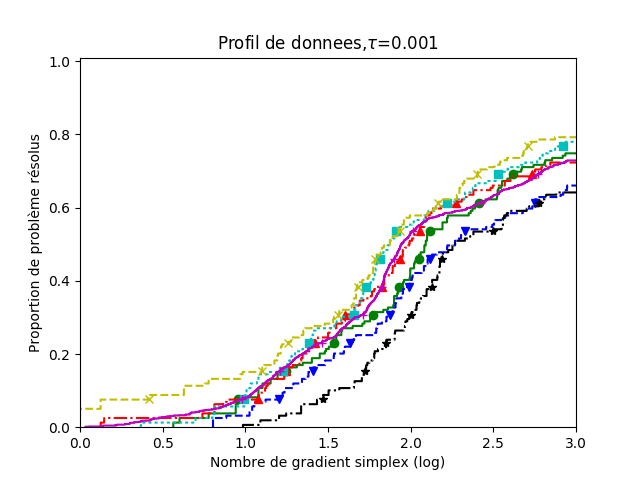
\includegraphics[width=\linewidth]{gog.png}
		\end{minipage}\\
		%
		%\begin{minipage}[t]{0.5\linewidth}
		%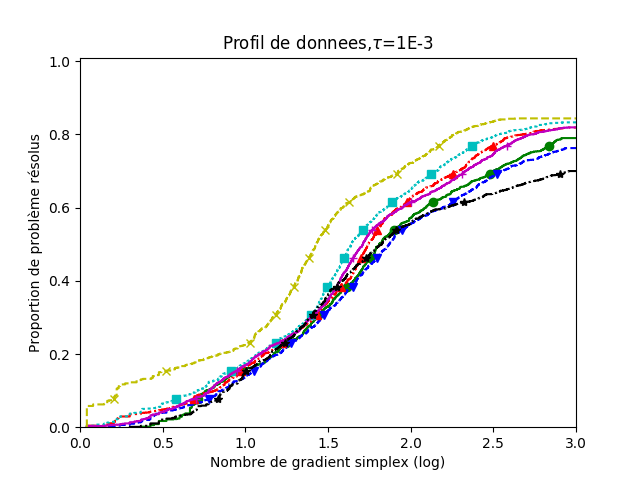
\includegraphics[width=\linewidth]{mog.png}
		%\end{minipage}
		
\includegraphics[width=\linewidth]{legende_mw.png}
		\vspace{-1em}
		\caption{\GPS~sur Moré-Wild}
		\vspace{-1.3em}
	\end{figure}
\end{center}
\begin{minipage}[t]{0.5\linewidth}
	\begin{enumerate}
		\pause
		\item Stratégie omnisciente moins dominante.
	\end{enumerate}
\end{minipage}%
\hfill%
\begin{minipage}[t]{0.5\linewidth}
	\begin{enumerate}
		\pause
		\item[\mynum{2}] Stratégie modèles performante.
		%\pause
		%\item[\mynum{3}] Impact moins important sur \MADS.
		%\pause
		%\item[\mynum{4}] Classement différent sur \CS~ et \MADS.
	\end{enumerate}
\end{minipage}
\end{frame}
%%%%%%%%%%%%%%%%%%%%%%%%%%%%%%%%%%%%%%%%%%%%%%%%%%%%%%%%%
%%%%%%%%%%%%%%%%%%%%%%%%%%%%% MADS %%%%%%%%%%%%%%%%%%%%%%
%%%%%%%%%%%%%%%%%%%%%%%%%%%%%%%%%%%%%%%%%%%%%%%%%%%%%%%%%
\begin{frame}
\frametitle{Comparaison des stratégies d'ordonnancement}
\noindent
\begin{center}
	\begin{figure}
		\vspace{-1em}
		\begin{minipage}[t]{0.5\linewidth}
			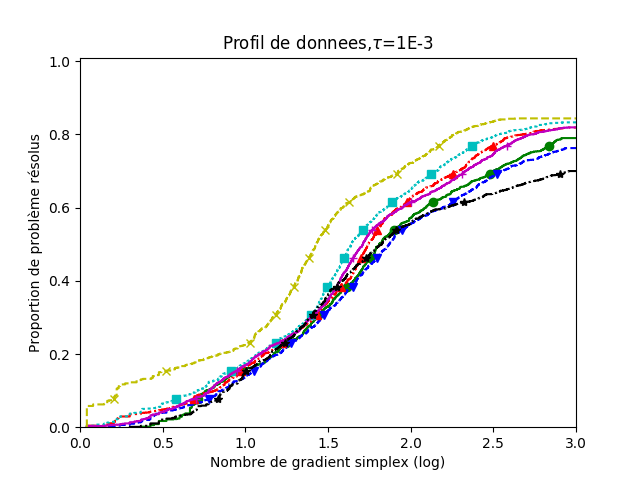
\includegraphics[width=\linewidth]{mog.png}
		\end{minipage}\\
		%
		%\begin{minipage}[t]{0.5\linewidth}
		%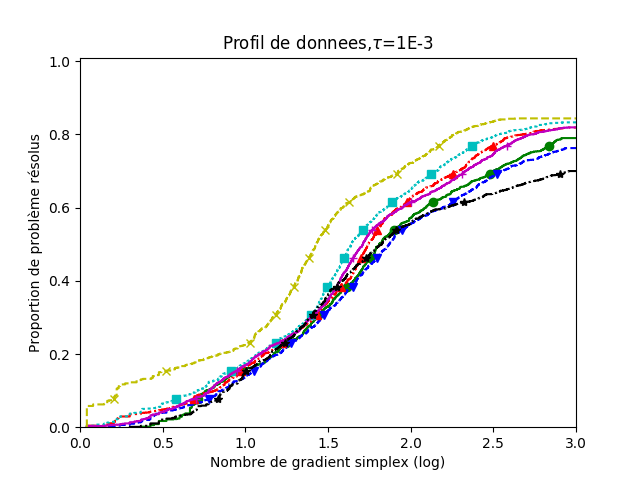
\includegraphics[width=\linewidth]{mog.png}
		%\end{minipage}
		
\includegraphics[width=\linewidth]{legende_mw.png}
		\vspace{-1em}
		\caption{\MADS~sur Moré-Wild}
		\vspace{-1.3em}
	\end{figure}
\end{center}
\begin{minipage}[t]{0.5\linewidth}
	\begin{enumerate}
		\pause
		\item Impact moins important sur \MADS.
	\end{enumerate}
\end{minipage}%
\hfill%
\begin{minipage}[t]{0.5\linewidth}
	\begin{enumerate}
		\pause
		\item[\mynum{2}] Classement différent sur \CS~ et \MADS.
		%\pause
		%\item[\mynum{3}] Impact moins important sur \MADS.
		%\pause
		%\item[\mynum{4}] Classement différent sur \CS~ et \MADS.
	\end{enumerate}
\end{minipage}
\end{frame}
%%%%%%%%%%%%%%%%%%%%%%%%%%%%%%%%%%%%%%%%%%%%%%%%%%%%%%%%%%%%%%%%
%%%%%%%%%%%%%%%%%%%%%%%%%%%%%% GSS %%%%%%%%%%%%%%%%%%%%%%%%%%%%%
%%%%%%%%%%%%%%%%%%%%%%%%%%%%%%%%%%%%%%%%%%%%%%%%%%%%%%%%%%%%%%%%
\begin{frame}
\frametitle{Comparaison des stratégies d'ordonnancement}
\noindent
\begin{center}
\begin{figure}
\vspace{-1em}
\begin{minipage}[t]{0.5\linewidth}
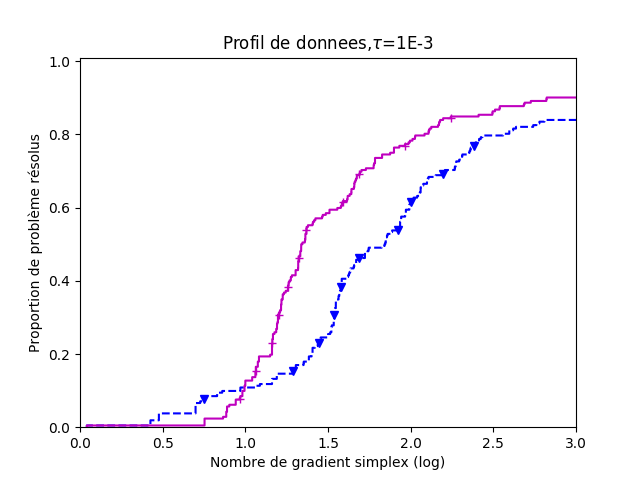
\includegraphics[width=\linewidth]{gss.png}
\end{minipage}\\
%%
%\hfill%
%\begin{minipage}[t]{0.5\linewidth}
%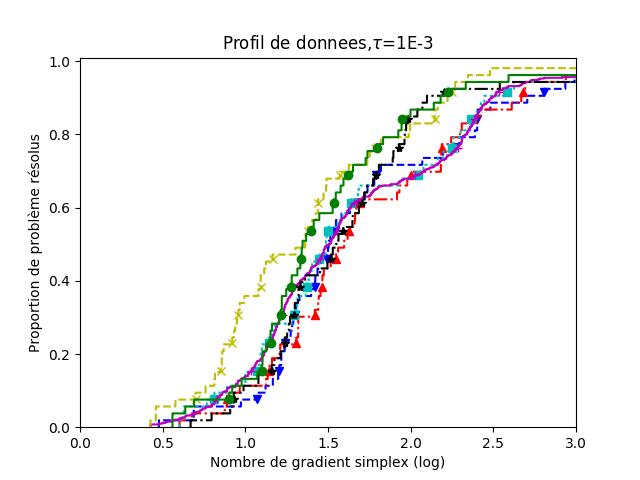
\includegraphics[width=\linewidth]{imfil.png}
%\end{minipage}

\includegraphics[width=\linewidth]{legende_gss.png}
\vspace{-1.5em}
\caption{\GSS~sur Moré-Wild}
\vspace{-1.3em}
\end{figure}
\end{center}
\begin{minipage}[t]{0.5\linewidth}
\begin{enumerate}
\pause
\item Stratégie aléatoire domine la stratégie lexicographique.
\end{enumerate}
\end{minipage}%
\hfill%
\begin{minipage}[t]{0.5\linewidth}
\begin{enumerate}
\pause
\item[\mynum{2}] Aucune autre stratégie disponible avec HOPSPACK.
\end{enumerate}
\end{minipage}
\end{frame}
%%%%%%%%%%%%%%%%%%%%%%%%%%%%%%%%%%%%%%%%%%%%%%%%%%%%%%%%
%%%%%%%%%%%%%%%%%%%%%%%% IMFIL %%%%%%%%%%%%%%%%%%%%%%%%%
%%%%%%%%%%%%%%%%%%%%%%%%%%%%%%%%%%%%%%%%%%%%%%%%%%%%%%%%
\begin{frame}
\frametitle{Comparaison des stratégies d'ordonnancement}
\noindent
\begin{center}
	\begin{figure}
		\vspace{-1em}
		\begin{minipage}[t]{0.5\linewidth}
			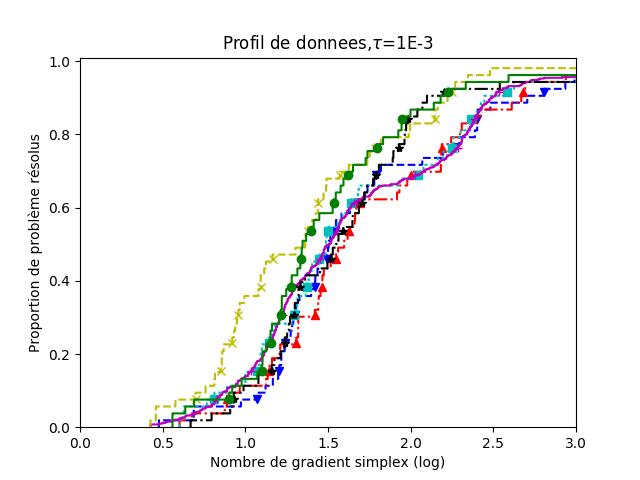
\includegraphics[width=\linewidth]{imfil.png}
		\end{minipage}\\
		%%
		%\hfill%
		%\begin{minipage}[t]{0.5\linewidth}
		%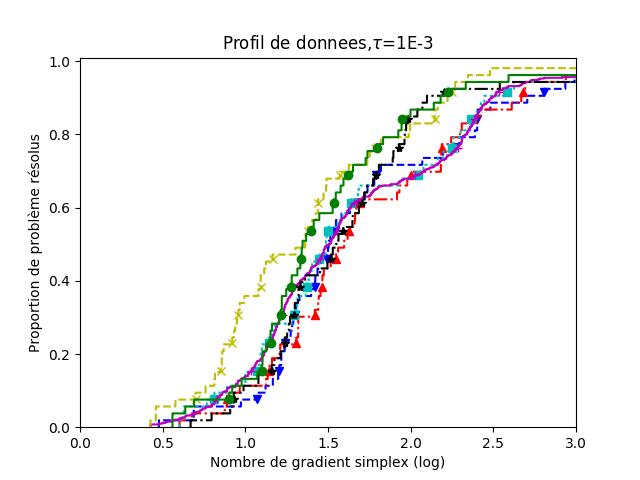
\includegraphics[width=\linewidth]{imfil.png}
		%\end{minipage}
		
\includegraphics[width=\linewidth]{legende_mw.png}
		\vspace{-1.5em}
		\caption{\IMFIL~sur Moré-Wild}
		\vspace{-1.3em}
	\end{figure}
\end{center}
\begin{minipage}[t]{0.5\linewidth}
	\begin{enumerate}
		\pause
		\item Opportunisme peut être profitable avec un ordonnancement omniscient.
	\end{enumerate}
\end{minipage}%
\hfill%
\begin{minipage}[t]{0.5\linewidth}
	\begin{enumerate}
		\pause
		\item[\mynum{2}] Avec les stratégies d'ordonnancement praticables, l'opportunisme est nuisible.
	\end{enumerate}
\end{minipage}
\end{frame}
%%%%%%%%%%%%%%%%%%%%%%%%%%%%%%%%%%%%%%%%%%%%%%%%%%%%%%%%
%%%%%%%%%%%%%%%%%%%%%% PROBLEMES CONTRAINTS%%%%%%%%%%%%%
%%%%%%%%%%%%%%%%%%%%%%%%%%%%%%%%%%%%%%%%%%%%%%%%%%%%%%%%
\begin{frame}
\frametitle{Comparaison des stratégies d'ordonnancement}
\noindent
\begin{center}
\begin{figure}
\vspace{-1em}
\begin{minipage}[t]{0.5\linewidth}
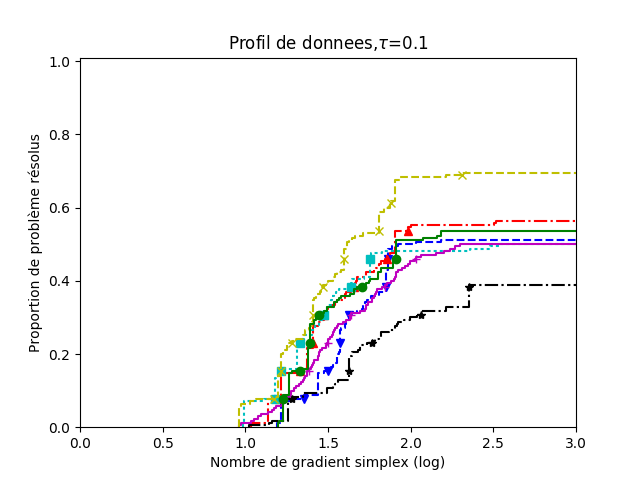
\includegraphics[width=\linewidth]{const.png}
\end{minipage}

\includegraphics[width=\linewidth]{legende_mw.png}
\vspace{-1.5em}
\caption{Problèmes contraints avec \MADS}
\vspace{-1.3em}
\end{figure}
\end{center}

\begin{center}
\begin{enumerate}
\pause
\item[\mynum{1}] Courbe de la stratégie omnisciente élevée.
\pause
\item[\mynum{2}] Stratégie réelles peu performantes.
\end{enumerate}
\end{center}

\end{frame}

\begin{frame}
\noindent
\begin{center}
\begin{figure}
\vspace{-1em}
\begin{minipage}[t]{0.5\linewidth}
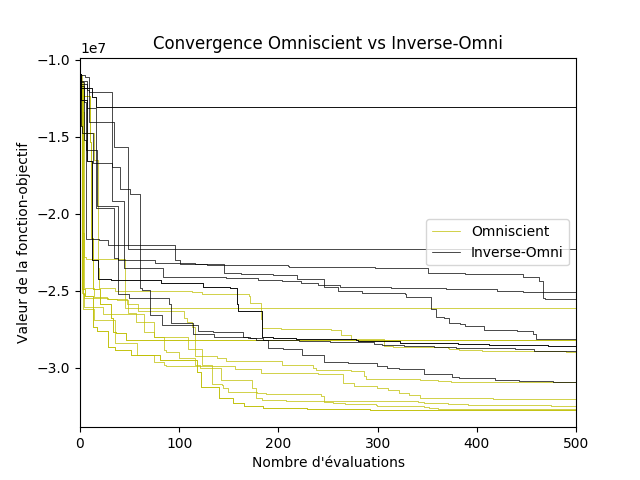
\includegraphics[width=\linewidth]{sty1.png}
\end{minipage}%
\hfill%
\begin{minipage}[t]{0.5\linewidth}
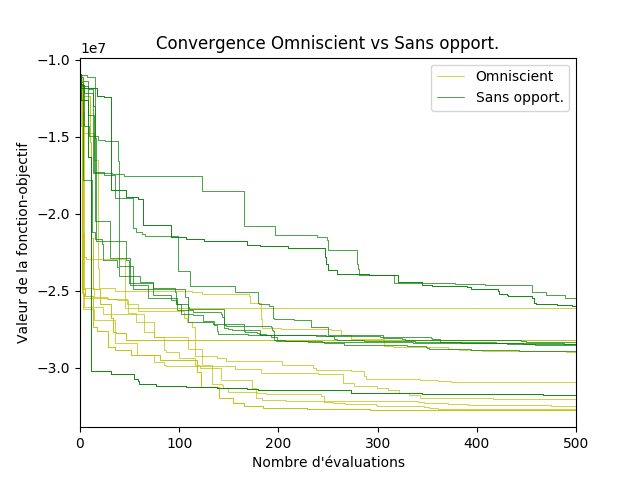
\includegraphics[width=\linewidth]{sty2.png}
\end{minipage}
\vspace{-1.5em}
\caption{Comparaison omnisciente, inverse-omnisciente et sonde complète}
\vspace{-1em}
\end{figure}
\begin{enumerate}
\pause
\item Stratégie omnisciente montre un impact de l'opportunisme sur STYRENE.
\pause
\item[\mynum{2}] Sonde complète ressemble d'avantage à inverse-omnisciente.
\end{enumerate}
\end{center}
\end{frame}

\begin{frame}
\noindent
\begin{center}
\begin{figure}
\vspace{-1em}
\begin{minipage}[t]{0.5\linewidth}
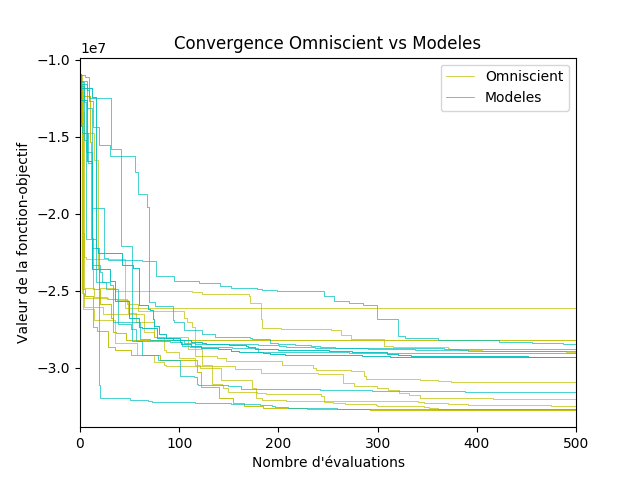
\includegraphics[width=\linewidth]{sty3.png}
\end{minipage}%
\hfill%
\begin{minipage}[t]{0.5\linewidth}
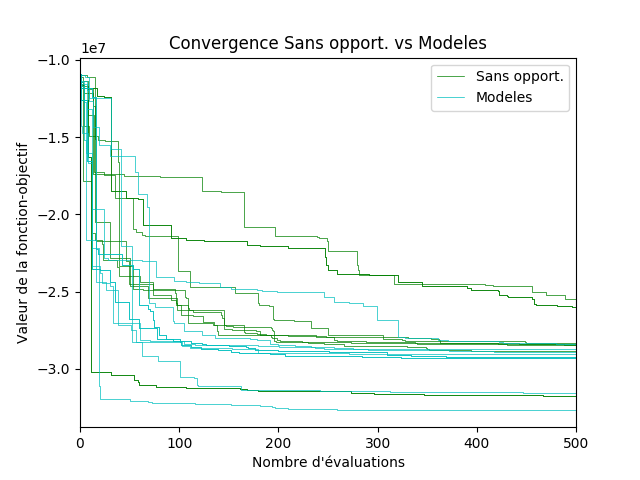
\includegraphics[width=\linewidth]{sty4.png}
\end{minipage}
\vspace{-1.5em}
\caption{Comparaison omnisciente, sonde complète et avec modèles}
\vspace{-1em}
\end{figure}
\begin{enumerate}
\pause
\item La stratégie avec modèles accélère la convergence si comparée à la sonde complète.
\pause
\item La stratégie avec modèles converge vers un moins bon optimum que la stratégie omnisciente.
\end{enumerate}
\end{center}
\end{frame}


\section{Conclusion}
\tableofcontents[currentsection,currentsubsection,subsectionstyle=show/hide]
\subsection{Conclusion}
\begin{frame}
\frametitle{Conclusion : Les grandes lignes}
\begin{itemize}
\item\only<1->{L'opportunisme est bénéfique aux méthodes de recherche directe directionnelles.}
\pause
\item\only<1>{~}\only<2->{L'opportunisme peut aussi être nuisible avec le mauvais ordonnancement.}
\pause
\item\only<1-2>{~}\only<3->{Plus la sonde est raffinée, moins son impact est important}
\pause
\item\only<1-3>{~}\only<4->{Stratégies autres que opportunisme simple $\rightarrow$ Sonde complète}
\pause
\item\only<1-4>{~}\only<5->{Classements des stratégies : Modèles, Aléatoires, Direction du dernier succès, sonde complète et lexicographique}
\pause
\item\only<1-5>{~}\only<6->{Pour \IMFIL, l'opportunisme est inutile ou nuisible}
\end{itemize}
\end{frame}

\begin{frame}
\frametitle{Conclusion : Suite?}
Il y a place à l'amélioration dans l'ordonnancement.
\pause
\begin{itemize}
\item\only<2->{Ordonnancer avec d'autre types de modèles que quadratiques}
\pause
\item\only<2>{~}\only<3->{Identifier d'autres stratégies d'ordonnancement (Distance à la solution d'un modèle, Distance à la cache).}
\pause
\item\only<2-3>{~}\only<4->{Identifier des stratégies avec la barrière progressive.}
\pause
\item\only<2-4>{~}\only<5->{Critère d'opportunisme : décroissance minimale}
\pause
\item\only<2-5>{~}\only<6->{Opportunisme et parallélisme?}
\end{itemize}
\end{frame}
%------------------------------------------------

%------------------------------------------------

\begin{frame}
\frametitle{Réferences}
\footnotesize{
	\begin{thebibliography}{99} % Beamer does not support BibTeX so references must be nserted manually as below
		\bibitem[J.J. Mor\'e and S.M. Wild 2009]{MoWi2009} J.J. Mor\'e and S.M. Wild (2009)
		\newblock   Benchmarking Derivative-Free Optimization Algorithms
		\newblock \emph{SIAM Journal on Optimization} 20(1). 172--191

		\bibitem[Audet, Tribes, 2017]{AuTr17} C. Audet and C. Tribes (2017)
		\newblock Mesh-based Nelder-Mead algorithm for inequality constrained
		optimization
		\newblock \emph{Les Cahiers du Gerad} G-2017-90.
		
		\bibitem[Audet, Béchard, Le Digabel 2008]{AuBeLe08}C. Audet and V. B\'echard and S. {Le~Digabel} (2008)
		\newblock Nonsmooth optimization through Mesh Adaptive Direct Search
		and Variable Neighborhood Search
		\newblock \emph{Journal of Global Optimization} 41-2.
		
		\bibitem[Le Digabel 2009]{Le09b} S. {Le~Digabel} (2009)
		\newblock Algorithm 909: NOMAD: Nonlinear Optimization with the MADS algorithm
		\newblock \emph{{ACM} Transactions on Mathematical Software} 37-4.
	\end{thebibliography}
}
\end{frame}


\end{document}
